\chapter{Have A Solid Plan (For Teens and Adults)}

These notes follow Jim Rohn's lecture as preserved in a curated LazyingArt LLC playlist rather than a clean institutional course. The order matters. The long autobiographical opening is not decoration; it is the lecture's way of earning the right to speak about agency, value, goals, and money. Only after the story of failure, mentorship, and later success does the talk condense into equations, comparison rules, and a compact plan for financial independence.

\section{Story, Failure, and the Teacher}

The lecture opens in the first person and stays there for a while. Rohn speaks to students by video because he cannot visit every school in person, and he uses that opening to explain why he thinks these principles deserve a hearing. He is not presenting a theory detached from life. He is presenting a sequence he believes changed his own life: poor choices, debt, humiliation, a teacher, new disciplines, and then a different economic result.

The biographical arc is sharp. He grows up in Idaho, leaves college early, marries young, starts a family, works hard, and still falls further behind. By age twenty-five he is, in his own description, nearly empty: pennies in his pocket, nothing in the bank, and embarrassed by promises he cannot keep. This is the point at which the lecture creates a genuine problem. Hard work alone is already present, so hard work cannot be the full explanation.

The turning point is the meeting with a wealthy mentor. The transcript varies in spelling, and we will write Mr.~Shouf for convenience. What matters is not merely that this man is rich, but that he is able to teach: books, disciplines, skills, language, personality, and the manner of changing oneself. Rohn presents the next five years as the first five years of a new life. By age thirty-one he is a millionaire. The talk therefore begins with a causal claim, not a boast.

The lecture condenses that claim into a sentence that functions almost like an axiom for everything that follows:
\begin{equation}
\text{If you change, everything will change for you.}
\end{equation}

We should notice the precision of the promise. The teacher does not say that the world will become kind, that politics will improve, or that luck will suddenly appear. He says that the locus of change must move inward. The lecture's later formulas are all expansions of this first statement.

\section{Wind, Sail, and the Location of Agency}

Before meeting Mr.~Shouf, Rohn says that he kept hoping for better conditions: a better boss, lower prices, a better tax structure, better circumstances. The teacher breaks that habit of thought with a governing metaphor. Economics, politics, and circumstance are the wind. The wind blows on everyone. The question is not whether we can stop the wind, but whether we can set a better sail.

The lecture does not write an equation here, but it plainly invites one:
\begin{equation}
\text{future outcome} = f(\text{wind},\text{sail-setting}).
\end{equation}
In the lecture's own language, the wind is the external world, and the sail is the internal arrangement of philosophy, skill, discipline, and judgment. A convenient companion notation is therefore
\begin{equation}
\text{wind} = \text{economics}+\text{politics}+\text{circumstance}, \qquad
\text{sail} = \text{philosophy}+\text{skill}+\text{discipline}.
\end{equation}
This is a reconstruction, not blackboard notation, but it captures the lecture's mechanism faithfully.

The point is not that the wind is irrelevant. On the contrary, America is described as unusually favorable wind: freedom, opportunity, and a wide economic ladder. But favorable wind by itself is still not enough. If we merely drift, then even good conditions do not reliably take us where we want to go.

That is why Rohn says he went to work not on the government, not on the company, and not on circumstances, but on himself. The first six years of his economic life ended in failure; the second six years, under the same broad wind, ended differently. The explanatory variable is not the weather. It is the sail.

\section{Personal Development, Value, and the Marketplace}

The first formal subject is personal development, and the lecture starts with money. That move is deliberate. Personal development can sound vague if we begin with slogans. Rohn begins instead with a measurable claim about the marketplace.

\subsection{Question \& Answer}

\paragraph{Question.} Do we get paid for time, or for value brought to the marketplace?

\paragraph{Answer.} The lecture's answer is crisp. Time is necessary, but time is not what is paid for. The relation is better written as
\begin{align}
\text{time} &\longrightarrow \text{value brought to the marketplace},\\
\text{pay} &\neq \text{time},\\
\text{therefore}\qquad \text{pay} &\propto \text{value brought to the marketplace}.
\end{align}

This is the first real derivation in the talk. It is not a technical economic model, but the logic is clear. If pay were literally for time, then equal time would guarantee equal pay, and one might as well stay home and have the money sent in. The lecture denies that picture explicitly. Equal time can yield very different results because what matters is the value carried into the marketplace during that time.

Once that statement is in place, the lecture asks a series of scaling questions. Can one become twice as valuable and earn twice as much in the same time? Three times? Five times? Ten times? The answer is yes each time. The point of the repetition is motivational, but the structure is real: value is the variable to be increased.

Rohn then gives a deliberately small example. The first step up the ladder is not mystical:
\begin{align}
\text{starting rung} &= \$5,\\
\text{next rung} &= \$6,\\
\Delta \text{ pay} &= \$1.
\end{align}
His comic illustration is that a person may be paid \$5 an hour to take out the trash, but if he whistles while doing it, he may be worth \$6. The lesson is not about music. It is about the smallest possible increment in attitude and presentation. The lecture does not wait for legislation to create the next rung. It says the next rung is already there.

\subsection{The Marketplace Ladder}

The talk briefly becomes diagrammatic at the easel. The board is only partly legible, so we must be careful. The safest use of the image is not as a verbatim transcription but as evidence for the lecture's layout: a comparison between non-market forms of value on one side and a vertical income ladder on the other.

\begin{figure}[t]
\centering

\includegraphics[width=0.78\linewidth]{lecture_09_figure_02.png}
\caption{Handwritten marketplace-value ladder on easel. The board is only partly legible, so it functions here as evidence for the lecture's comparison layout rather than as a fully readable derivation.}
\end{figure}

The right side of the board supports the transcript's ladder:
\begin{equation}
\$5 < \$50 < \$500 < \$80\,\text{million}.
\end{equation}
The precise handwriting is uncertain, but the structure is secure: a low rung, higher hourly rungs, and a very high top compensation.

Nearby, we keep a cautious redraw. It is a reading aid, not a replacement for the screenshot.

\begin{figure}[t]
\centering
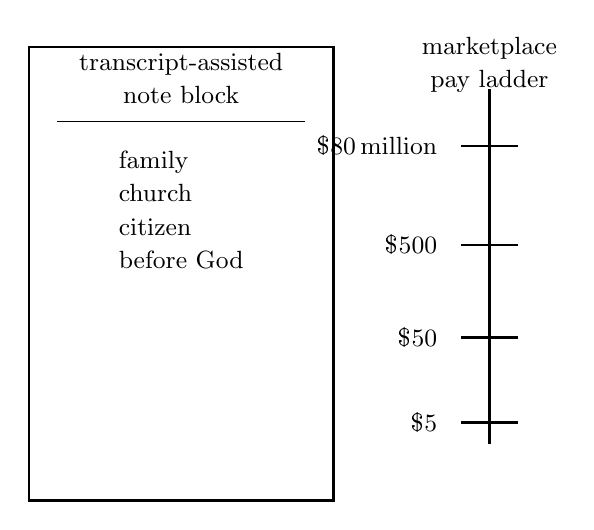
\begin{tikzpicture}[x=0.9cm,y=0.9cm]
\draw[thick] (0,0) rectangle (4.3,6.4);
\node[align=center] at (2.15,5.95) {\small transcript-assisted\\\small note block};
\draw (0.4,5.35) -- (3.9,5.35);
\node[align=left] at (2.15,4.1) {\small family\\\small church\\\small citizen\\\small before God};

\draw[thick] (6.5,0.8) -- (6.5,5.8);
\draw[thick] (6.1,1.1) -- (6.9,1.1);
\draw[thick] (6.1,2.3) -- (6.9,2.3);
\draw[thick] (6.1,3.6) -- (6.9,3.6);
\draw[thick] (6.1,5.0) -- (6.9,5.0);

\node[left] at (5.9,1.1) {\small \$5};
\node[left] at (5.9,2.3) {\small \$50};
\node[left] at (5.9,3.6) {\small \$500};
\node[left] at (5.9,5.0) {\small \$80\,million};

\node[align=center] at (6.5,6.15) {\small marketplace\\\small pay ladder};
\end{tikzpicture}
\caption{Cautious redraw of the board structure. The right ladder is the secure part. The left block is transcript-assisted and generic because the handwriting itself is not fully legible.}
\end{figure}

The lecture immediately adds an important restraint. Marketplace value is not the same thing as total human worth:
\begin{equation}
\text{human/social value} \not\equiv \text{marketplace value}.
\end{equation}
A person may be valuable as a brother, a member of a family, a member of a church, a citizen, or in the sight of God, and yet not be very valuable \emph{to the marketplace}. The economic ladder is therefore only one ordering. It is not a total ordering of the person.

The practical conclusion is the sentence Rohn says made sense to him at once: work harder on yourself than you do on your job. In the lecture's logic, that is the operative rule for climbing the ladder.

\section{Experience, OPE, Books, and Journals}

Once the lecture has defined value economically, it widens personal development into a method of learning. Here the rhythm is cumulative rather than deductive. Each layer adds another channel by which the self can be altered.

The first channel is personal experience. Learn from what happens to us. Correct what went badly in the last month or the last year. The teacher's summary is wonderfully severe: if what we have been doing is not working, we should not keep doing it. The lecture is not sentimental about failure. It asks that failure be converted into information.

The second channel is what Rohn abbreviates as OPE, other people's experiences. This includes both failures and successes. In principle we should learn from both. The speaker jokes that failures rarely give seminars, but the point stands: there is no reason to pay full tuition for every mistake ourselves if another life has already displayed the same pattern.

He then breaks this borrowed learning into a sequence:
\begin{enumerate}
\item observation,
\item listening,
\item reading,
\item journaling.
\end{enumerate}
Observation means watching successful people in sports, business, or other fields and noting their disciplines. Listening means lectures, sermons, classes, and recorded talks. Reading means books, not as decoration, but as a long accumulation of other people's distilled experience. Journaling is the final step because it turns passing impressions into retained capital.

There is a small but important structure here:
\begin{equation}
\text{heard or seen value} \longrightarrow \text{written note} \longrightarrow \text{later review} \longrightarrow \text{usable value}.
\end{equation}
Again, this is companion notation rather than the lecturer's own formula, but it captures the process exactly. The journal is the device by which fleeting insight becomes something we can return to.

This matters because the lecture is trying to make self-development concrete. It is not merely ``be better.'' It is: read, listen, observe, write, review, and thereby change the available material out of which future action will be made.

\section{Goals: Past as School, Future as Promise}

The second major subject is goal-setting, and the lecture begins by reorganizing time. First the past: the past is not to be carried as a burden or used as a club against ourselves. It is to be treated as a school. That is already a strong adjustment in attitude. The past becomes instruction rather than weight.

Then the lecture turns to the future. The future, Rohn says, is the promise. We are not yet in the technical part of goals. We are still in the motivational foundation that makes goals possible.

\subsection{Question \& Answer}

\paragraph{Question.} Why do most people face the future with apprehension instead of anticipation?

\paragraph{Answer.} Because the future is usually left undesigned. The lecture's contrast can be written compactly as
\begin{equation}
\text{future not designed} \Rightarrow \text{apprehension}, \qquad
\text{future well designed} \Rightarrow \text{anticipation}.
\end{equation}

This is one of the lecture's sharpest local tensions. The future by itself is not the problem. What matters is whether it has been given shape. If it remains vague, it becomes threatening. If it is specified, it becomes attractive.

The talk then moves into a practical sequence. Goal-setting is not presented as mystical visualization. It is almost embarrassingly simple:
\begin{enumerate}
\item decide what we want,
\item write it down,
\item keep the old lists,
\item check things off.
\end{enumerate}
The simplicity is part of the lecture's strategy. Rohn is trying to remove excuses. One need not begin with an advanced system; one needs paper, thought, and seriousness.

The anecdote about Spain belongs here. The transcript is rough in places, but the secure core is clear. He had long set the goal of going to Spain, and when the plane touched down in Madrid, he checked the goal off in his journal. That is not a deep piece of mathematics, but it is a precise example of the lecture's attitude toward design: the future should become concrete enough that its realization can be marked.

\section{Promise, Price, and What Goals Make of Us}

At this point the lecture could easily collapse into acquisition, but it does not. Rohn adds two linked corrections. The first is that every promise has a price. The second is that the deeper value of a goal lies in what it makes of us.

The price principle is the lecture's next compact law:
\begin{equation}
\text{promise clarity}\uparrow \Rightarrow \text{price difficulty}\downarrow.
\end{equation}
The price does not disappear. Classes must still be taken, books must still be read, disciplines must still be accepted. But the subjective burden changes when the promise is vivid. A clear future makes present cost easier to bear.

This is exactly why the talk places goals after personal development but before the money formula. Without a designed future, discipline feels arbitrary. With a designed future, discipline becomes intelligible.

The lecture then intensifies the point with the millionaire example. The teacher advises the young Rohn to set a goal to become a millionaire, but not chiefly because a million dollars would be pleasant to possess. The more important reason is what the process would require him to become. The lecture later verifies that claim through loss. By thirty-one he is a millionaire; by thirty-three he is broke again. The teacher is vindicated because the money was not the deepest asset. The more valuable residue was the transformed person: the skills, the understanding of the marketplace, the language, the habits.

We may say, in the lecture's spirit, that the invariant is not the cash balance but the enlarged self. That is why goals must be neither too low nor morally corrupt. If they are too low, they do not force growth. If they demand the sale of character, they are self-defeating. The lecture wants a middle road: goals large enough to require change, but not so distorted that they destroy the person who achieves them.

\section{Financial Independence and the Dollar Formula}

Only after all of this preparation does the lecture turn to its most formula-like part. The phrase itself is carefully chosen. Rohn prefers \emph{financial independence} to the more emotionally loaded language of becoming rich.

\begin{definition}
Financial independence is the ability to live from the income of your own personal resources.
\end{definition}

The talk immediately converts that verbal definition into a threshold condition:
\begin{equation}
\text{income from personal resources} \ge \text{required living expense}.
\end{equation}
No detailed finance theory is supplied, and none should be imported. This is a lecture maxim, not a textbook model. Still, the logic is plain: when resource-generated income covers the chosen way of living, dependence on wages has been reduced or overcome.

The time horizon is then stated explicitly:
\begin{equation}
15 \to 35 = 20\ \text{years}.
\end{equation}
The speaker's claim is that twenty years is enough time, in America and with the right plan, to reach financial independence. If one fails, the lecture says, the first place to look is not the country but the plan.

The plan begins with philosophy:
\begin{align}
\text{poor philosophy} &: \text{spend first, invest what is left},\\
\text{rich philosophy} &: \text{invest first, spend what is left}.
\end{align}
The lecture insists that the amount matters less than the order. The sequence of operations is itself the decisive act of philosophy.

This leads to the dollar formula:
\begin{equation}
1.00 = 0.70 + 0.10 + 0.10 + 0.10.
\end{equation}

\begin{table}[t]
\centering
\begin{tabular}{ll}
$0.70$ & spending \\
$0.10$ & charity \\
$0.10$ & active capital \\
$0.10$ & passive capital
\end{tabular}
\caption{The lecture's dollar-allocation rule, stated as a compact working formula rather than as formal finance theory.}
\end{table}

The first tenth is generosity. The second is active capital, money used to produce profit directly. The third is passive capital, money lent or entrusted to others so that it yields interest and, in the lecture's terms, compound interest over time. The talk names compound interest but does not derive a formula for it; the important point is qualitative rather than algebraic.

Rohn also gives an explicit worked example of active capital:
\begin{align}
\text{purchase of broken wagon} &= \$1,\\
\text{sale after repair} &= \$5,\\
\text{profit} &= \$4.
\end{align}
This is a child-sized business model, but that is exactly the point. The lecture wants the principle to begin small and early. Capital is not reserved for large institutions. It can begin as a single dollar turned into a repaired object and then into profit.

The lecture compresses its ranking of economic paths into two maxims:
\begin{equation}
\text{profits} > \text{wages}, \qquad \text{borrower} < \text{lender}.
\end{equation}
These are not rigorous inequalities; they are lecture shorthand for position and power. Wages make a living, profits make a fortune. The borrower is servant to the lender, and therefore the lender occupies what the speaker calls the power position.

The final move inside this section is unexpectedly psychological. Rohn returns to attitude. Paying bills and paying taxes are reinterpreted. To pay \$100 on a debt is not merely to lose \$100; it is to reduce liabilities. Taxes are placed within the system that feeds the goose that lays the golden eggs. The lecture therefore refuses to let the formula remain mechanical. The plan must be carried by an attitude capable of sustaining it.

\section{Summary}

The lecture begins with a broke twenty-five-year-old and ends with four questions to ponder. Between those poles it builds a compact sequence.

First, change the self rather than waiting for the wind to improve. Second, understand pay through value brought to the marketplace rather than through time alone. Third, learn systematically: from our own mistakes, from other people's experiences, from books, and from journals. Fourth, design the future clearly enough that the price of discipline becomes payable. Fifth, give the dollar an order: spend less than all of it, give part away, turn part into active capital, and turn part into passive capital.

The closing questions should remain visible because they are not ornaments. They are the lecture's final compression of its whole argument:
\begin{enumerate}
\item Why?
\item Why not?
\item Why not you?
\item Why not now?
\end{enumerate}
The chapter has no formal proof in the mathematical sense. What it has instead is a chain of lecture maxims, examples, and small equations whose function is to relocate agency, sharpen intention, and turn ambition into a plan.